\documentclass[kravspec/krav.tex]{subfiles}

\begin{document}

\section{Översikt av systemet}
Här beskrivs produkten övergripande där generella krav ställs på produkten och
dess avgränsningar.
\begin{figure}[h]
    \centering
    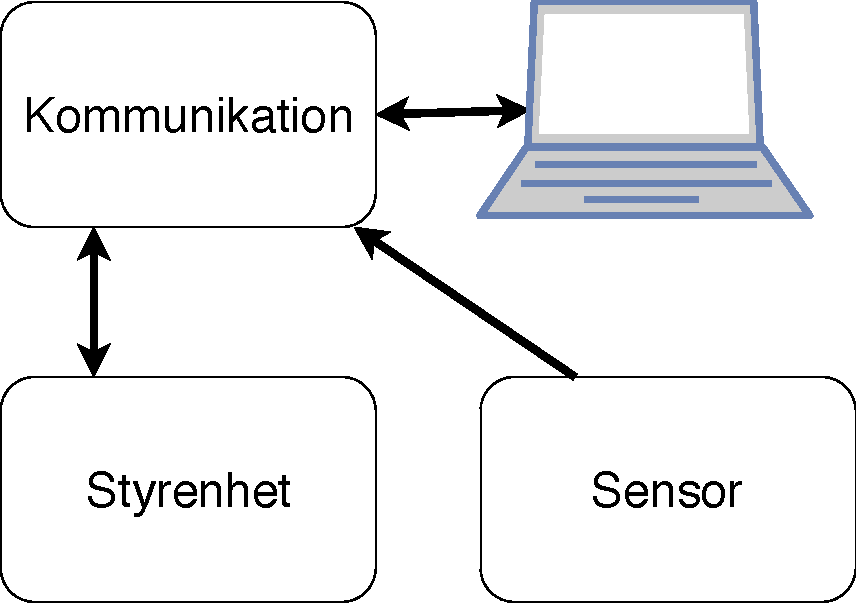
\includegraphics[width=0.6\linewidth]{kravspec/figures/overview-schema.pdf}
    \caption{Övergripande bild över systemet och dess moduler.}
    \label{fig:overview}
\end{figure}

\subsection{Grov beskrivning av produkten}
Produkten är en bil med fyra hjul som ska med hjälp av ett känt vägnät ta sig
till en passagerare och skjutsa passageraren till önskad destination. Den här
bilen ska kunna åka framåt, bakåt, svänga vänster och höger. Bilen kommer ha
en kamera som tar bilder från en riktning eller flera.  Bland annat ska
man kunna initiera en bluetooth-länk mellan bilen och en dator som har stöd för
bluetooth. Bilen ska ha ett läge där man kan fjärrstyra bilen och ett läge där
bilen ska köra autonomt i vägnätet samt undvika hinder.

\subsection{Produktkomponenter}
Lämplig hårdvara med kompletterande mjukvara kommer finnas i den kompletta
produkten. Bland annat ska även tekniskt dokumenation ingå i produkten.

\subsection{Beroenden till andra system}
Fjärstyrning av bilen skall vara beroende av en dator som har stöd för
bluetooth. Det autonoma läget aktiveras från användargränsnittet tillgänglig på
datorn med bluetooth. Kameran kommer vara beroende till en mikroprocessor som
ingår i systemet.

\subsection{Ingående delsystem}
Systemet ska bestå av delsystem enligt figur \ref{fig:overview}. Sensormodulen
ska hämta data om omgivningen, bland annat en sensor som mäter avstånd till
objekt i omgivning och tejpföljare som sensorer. Lämplig data av omgivning
skickas till kommunikationsmodell. Produkten har även en styrmodul som ser till
att bilen kan styras beroende på data från kommunikationsmodul.

\subsection{Avgränsningar}
Små väghinder som låga grova vägkanter och gropar tas ej hänsyn till. Vägen
förväntas bestå av hinder som är fördefinierade i banspecifikationen. Vägen
antas vara plan utan gropar och markerad med tejp. Parkeringsfickan förväntas
vara markerad med en specifik färg som skiljer sig från färgen på
vägmarkeringarna.

\subsection{Generella krav på hela systemet}
Nedan följer de generella krav som taxin ska eller bör uppfylla.  Kraven har
vardera en prioritet där 1 motsvarar något som skall vara klart och 2 att det
vore önskvärt att det är avklarat.

\setcounter{reqcat}{1}
\begin{reqlist}
    \req{Taxin ska kunna skicka aktuell mätdata till den bärbara datorn.
    Mätdata inkluderar avstånd till vägkant, avstånd till hinder, avlagd
    sträcka, styrbeslut och motorernas styrning.}
    \req{Det ska finnas ett användargränssnitt på den bärbara datorn som visar
    mätdata mottaget från taxin.}
    \req{Banans vägnät skall kunna matas in via användargränssnittet och
    därefter användas av taxin för att navigera banan.}
    \req{Användargränssnittet skall visa en karta över banans vägnät.}
    \req{Under körning skall positionsdata fortlöpande skickas till en bärbar
    dator och visas på användargränssnittets karta.}
    \req{Användaren skall kunna växla mellan autonom och manuell körning via
    användargränssnittet.}
    \req{Successiv inmatning av reglerparametrarna skall vara möjlig via
    användargränssnittet.}
    \req{Bilen skall kunna fjärrstyras via användargränssnittet. Kommandon
    inkluderar köra framåt, bakåt, stanna och svänga vänster eller höger.}
    \req{Under autonom körning ska taxin kunna köra från en punkt till en annan
    i ett känt tvåfiligt vägnät.}
    \req{Under autonom körning skall bilen navigera vägnätet enligt
    högertrafik.}
    \req{Under autonom körning skall bilen stanna ifall hinder befinner sig på
    vägen, tills hindret är borta.}
    \reqspec{original}{2}{Bilen ska kunna köra om ett hinder istället för att
    stanna, om det sker utan att bryta mot trafikregler.}
    \req{Under autonom körning skall bilen navigera genom vägnätet från en
    förutsatt position till en annan förutsatt destination.}
    \req{Bilen skall kunna stanna vid en stopplinje}
    \req{Bilen skall kunna svänga av in i en parkeringsficka och stanna där.}
    \req{Bilen skall klara av att navigera i rondeller där högertrafik gäller.}
    \reqspec{original}{2}{Bilen skall kunna delta i en tävling där tiden för
    varje uppdrag mäts.}
    \reqspec{original}{2}{Bilen skall aktivera blinkers vid svängning samt
    hämtning och avlämning.}
    \req{Bilen ska vara moduluppbyggd där varje modul innehåller en egen
    processor. En kommunikationsmodul, en styrmodul samt en sensormodul skall
    ingå.}
    \req{Bilen skall ha en kamera som tar bilder åtminstone åt en riktning.}
    \reqspec{original}{2}{Direktsändning av kamerabilden skall visas på en
    bärbar dator.}
    \req{Bilen ska använda sig av en styralgoritm så att den föredrar att
    befinna sig centralt i filen.}
\end{reqlist}

\end{document}
